\documentclass[convert={density=300,outext=.png}]{standalone}
\usepackage{tikz}
\usetikzlibrary{shapes,arrows,decorations,decorations.pathmorphing,arrows.meta,patterns,decorations.markings}

\begin{document}
%% Use \usepackage{tikz}
%% Use \usetikzlibrary{shapes,arrows,decorations, decorations.pathmorphing,arrows.meta,patterns}
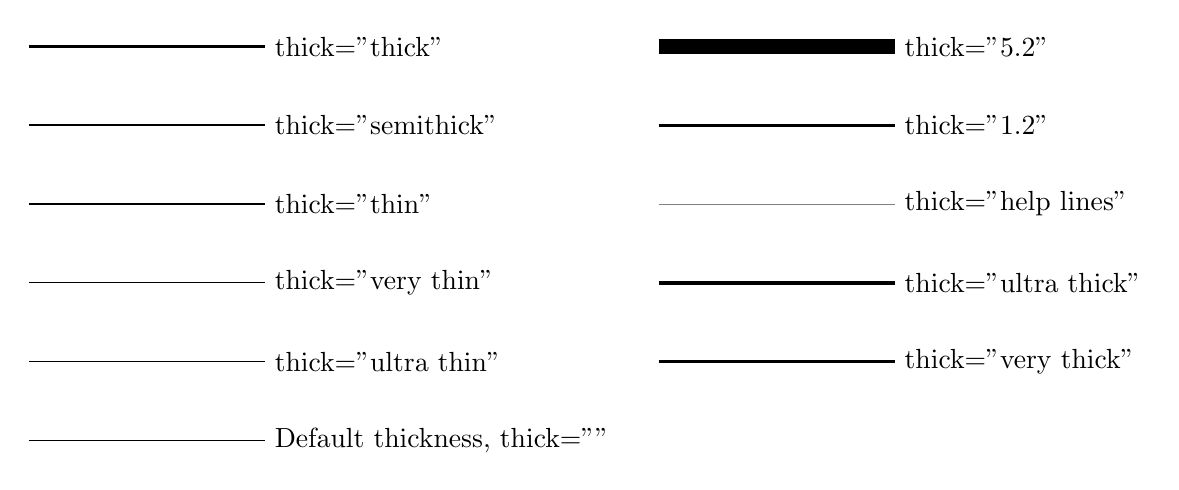
\begin{tikzpicture}[scale=1.0000]
	\tikzstyle{every node}=[scale=1.0000]
	
	%%Created with tikzpy
	
	\draw  (0.0000,0.0000,0.0000) -- (3.0000,0.0000,0.0000);
	\node [right]  at (3.0000,0.0000,0.0000)  {Default thickness, thick=""};
	\draw [ultra thin]  (0.0000,1.0000,0.0000) -- (3.0000,1.0000,0.0000);
	\node [right]  at (3.0000,1.0000,0.0000)  {thick="ultra thin"};
	\draw [very thin]  (0.0000,2.0000,0.0000) -- (3.0000,2.0000,0.0000);
	\node [right]  at (3.0000,2.0000,0.0000)  {thick="very thin"};
	\draw [thin]  (0.0000,3.0000,0.0000) -- (3.0000,3.0000,0.0000);
	\node [right]  at (3.0000,3.0000,0.0000)  {thick="thin"};
	\draw [semithick]  (0.0000,4.0000,0.0000) -- (3.0000,4.0000,0.0000);
	\node [right]  at (3.0000,4.0000,0.0000)  {thick="semithick"};
	\draw [thick]  (0.0000,5.0000,0.0000) -- (3.0000,5.0000,0.0000);
	\node [right]  at (3.0000,5.0000,0.0000)  {thick="thick"};
	\draw [very thick]  (8.0000,1.0000,0.0000) -- (11.0000,1.0000,0.0000);
	\node [right]  at (11.0000,1.0000,0.0000)  {thick="very thick"};
	\draw [ultra thick]  (8.0000,2.0000,0.0000) -- (11.0000,2.0000,0.0000);
	\node [right]  at (11.0000,2.0000,0.0000)  {thick="ultra thick"};
	\draw [help lines]  (8.0000,3.0000,0.0000) -- (11.0000,3.0000,0.0000);
	\node [right]  at (11.0000,3.0000,0.0000)  {thick="help lines"};
	\draw [line width = 1.2000]  (8.0000,4.0000,0.0000) -- (11.0000,4.0000,0.0000);
	\node [right]  at (11.0000,4.0000,0.0000)  {thick="1.2"};
	\draw [line width = 5.2000]  (8.0000,5.0000,0.0000) -- (11.0000,5.0000,0.0000);
	\node [right]  at (11.0000,5.0000,0.0000)  {thick="5.2"};

\end{tikzpicture}
\end{document}
